\chapter{Detalles de implementación y resultados computacionales}\label{chapter:implementation}

Los experimentos y resultados obtenidos de estos son esenciales para la validaci\'on del modelo computacional que se desarrolla. En esta sección se presentan los resultados obtenidos luego de promediar varias simulaciones del autom\'ata, alrededor de unas 30. Se llevan a cabo en un ordenador de gama media-alta con un i3de 8va generaci\'on con un reloj a 2.20GHz y 12gb de RAM. Se mencionaron algunas de las configuraciones que se aplicaron en el cap\'itulo anterior, pero en este se suministran las restantes.

\begin{table}[!ht]
    \begin{center}
    \scalebox{0.9}{\begin{tabular}{|p{2cm}|p{14.5cm}|}\hline
    \emph{Red} & $s_x=200$; $s_y=100$; $s_z=100$; $s_o=100$; $p = 0$.$01$. \\\hline
    
    \emph{Estados} & Para el \'organo primario correspondiente con la mama -- Esquema I: $v_x^t=50$, $v_y^t=50$, $v_z^t=50$. Para el \'organo secundario correspondiente con el pulm\'on -- Esquema I: $o_s=100$.\\\hline 
    
    \emph{Nutrientes} & Para el \'organo primario -- $R_1 = \lbrace v~|~v \in V(G) : (0 \leq v_x < 100) \wedge (0 \leq v_y < 50) \wedge (0 \leq v_z < 50) \rbrace$, $B_{01}=\lbrace \overrightarrow{\nu_{((0,0),(0,1))}} \rbrace$, $R_2 = \lbrace v~|~v \in V(G) : (0 \leq v_x < 100) \wedge (50 \leq v_y < 100) \wedge (50 \leq v_z < 100) \rbrace$. Para el \'organo secundario -- $R_3 = \lbrace v~|~v \in V(G) : (100 \leq v_x < 200) \wedge (0 \leq v_y < 100) \wedge (0 \leq v_z < 100) \rbrace$.\\\hline
    \end{tabular}}\vspace*{-0.5cm}
    \end{center}
    \caption[Valores de los par\'ametros de construcci\'on de la red, de la asignaci\'on de estados iniciales y de las regiones y vectores de nutrientes]{Valores de los par\'ametros de construcci\'on de la red, de la asignaci\'on de estados iniciales y de las regiones y vectores de nutrientes. Se utiliza la escala $1:3$ donde el tiempo transcurrido entre las generaciones del aut\'omata $n$ y $n+1$ se corresponde a $72$ horas y cada celda del aut\'omata contiene $9$ c\'elulas reales.}
    \label{table-net-params}
    \end{table}


\section{Crecimiento avascular}
\label{sec-avascular-results}

Primeramente se tiene en cuenta describen el desarrollo de un tumor avascular de crecimiento r\'apido. Al final de cada sección se comparan los resultados con \cite{viabarre2019}.Para ello se utilizan los valores de la poblaci\'on inicial y de las capacidades de carga m\'inimas, promedio y m\'aximas correspondientes con el intervalo de radios avasculares $R_a \in [0$.$5, 1]mm$ y una probabilidad m\'axima avascular $\rho_{max}^a=1$ como se muestran en el cuadro~\ref{table-avascular}

\begin{table}[!ht]
\begin{center}
\scalebox{0.9}{\begin{tabular}{|p{2.1cm}|p{14.5cm}|}\hline
\emph{M\'inimo} & $P_0^a=1$, $K_a=6$.$944 \times 10^1$, $r_a=5$.$797 \times 10^{-2}$, $\Delta t=1$.$693 \times 10^1$, $n_a=9$, generaciones del aut\'omata: $10$~($30$ d\'ias). \\\hline
\emph{Promedio} & $P_0^a=1$, $K_a=2$.$222 \times 10^2$, $r_a=1$.$802 \times 10^{-2}$, $\Delta t=2$.$996 \times 10^1$, $n_a=20$, generaciones del aut\'omata: $21$~($63$ d\'ias).\\\hline
\emph{M\'aximo} & $P_0^a=1$, $K_a=4$.$938 \times 10^2$, $r_a=8$.$097 \times 10^{-3}$, $\Delta t=4$.$558 \times 10^1$, $n_a=34$, generaciones del aut\'omata: $35$~($105$ d\'ias).\\\hline
\end{tabular}}\vspace*{-0.6cm}
\end{center}
\caption[Par\'ametros del desarrollo de un carcinoma ductal infiltrante de crecimiento r\'apido durante la etapa avascular]{Par\'ametros del desarrollo de un carcinoma ductal infiltrante de crecimiento r\'apido durante la etapa avascular.}
\label{table-avascular}
\end{table}

Para realizar la comparaci\'on con un carcinoma ductal que crezca m\'as lento se utilizan los valores de la poblaci\'on inicial y de las capacidades de carga m\'inimas, promedio y m\'aximas correspondientes con el intervalo de radios avasculares $R_a \in [0$.$5, 1]mm$ y una probabilidad m\'axima avascular $\rho_{max}^a=0$.$1$ como se muestra en el cuadro~\ref{table-avascular-1}.

\begin{table}[!ht]
    \begin{center}
    \scalebox{0.9}{\begin{tabular}{|p{2.1cm}|p{14.5cm}|}\hline
    \emph{M\'inimo} & $P_0^a=1$, $K_a=6$.$944 \times 10^1$, $r_a=5$.$797 \times 10^{-3}$, $\Delta t=2$.$854 \times 10^1$, $n_a=51$, generaciones del aut\'omata: $52$~($156$ d\'ias).\\\hline
    \emph{Promedio} & $P_0^a=1$, $K_a=2$.$222 \times 10^2$, $r_a=1$.$802 \times 10^{-3}$, $\Delta t=5$.$497 \times 10^1$, $n_a=109$, generaciones del aut\'omata: $110$~($330$ d\'ias).\\\hline
    \emph{M\'aximo} & $P_0^a=1$, $K_a=4$.$938 \times 10^2$, $r_a=8$.$097 \times 10^{-4}$, $\Delta t=8$.$604 \times 10^1$, $n_a=178$, generaciones del aut\'omata: $179$~($537$ d\'ias).\\\hline
    \end{tabular}}\vspace*{-0.6cm}
    \end{center}
    \caption[Par\'ametros del desarrollo de un carcinoma ductal infiltrante de crecimiento lento durante la etapa avascular]{Par\'ametros del desarrollo de un carcinoma ductal infiltrante de crecimiento lento durante la etapa avascular.}
    \label{table-avascular-1}
    \end{table}

% Imagenes con funciones
\begin{figure}[p]
    \begin{center}
    \subfigure[Crecimiento m\'inimo $K_a=6$.$944 \times 10^1$]{\scalebox{0.4}{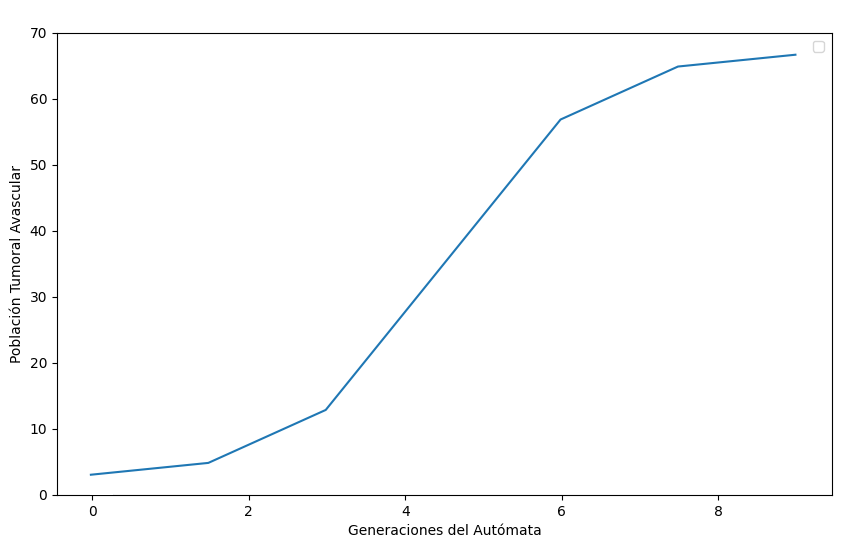
\includegraphics{img/automata/1.1.1.png}}}
    \subfigure[Crecimiento promedio $K_a=2$.$222 \times 10^2$]{\scalebox{0.4}{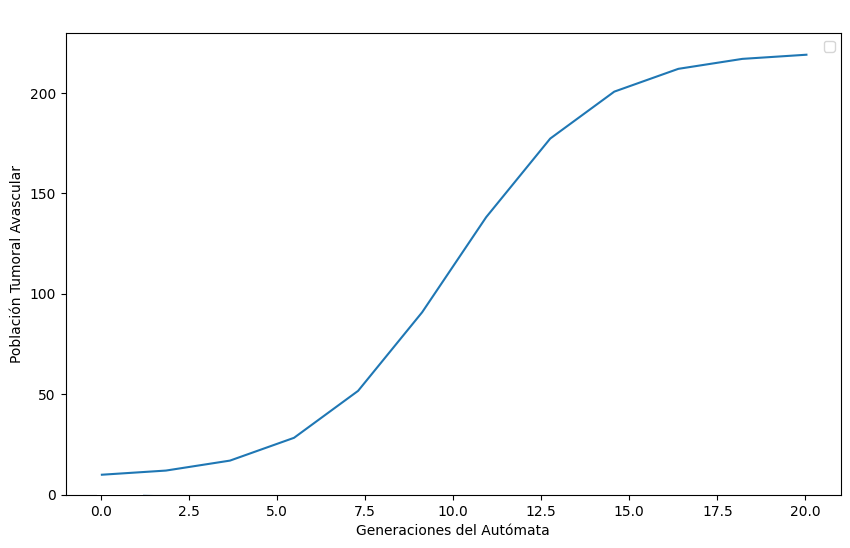
\includegraphics{img/automata/2.2.2.png}}}
    \subfigure[Crecimiento m\'aximo $K_a=4$.$938 \times 10^2$]{\scalebox{0.4}{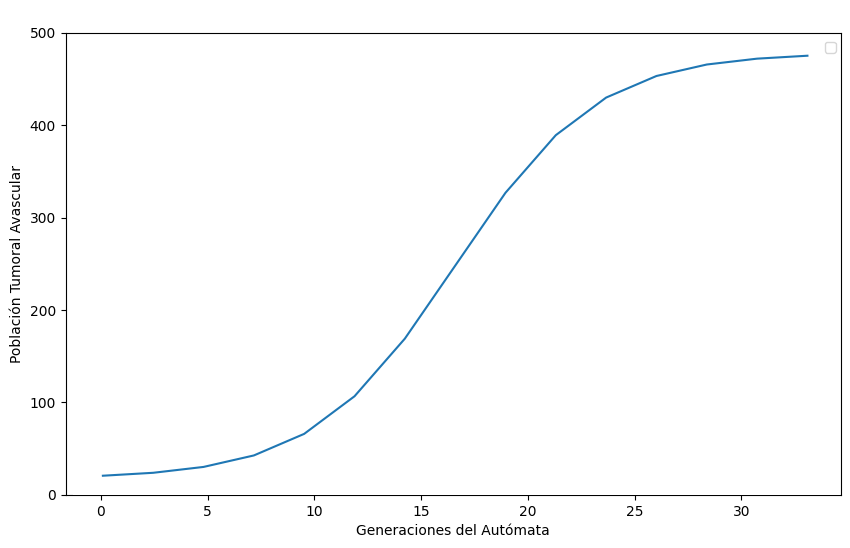
\includegraphics{img/automata/3.3.3.png}}}
    \end{center}\vspace*{-0.6cm}
    \caption[Poblaci\'on y radios de un carcinoma ductal infiltrante de crecimiento r\'apido con $\rho_{max}^a=1$ durante la etapa avascular]{Poblaci\'on de un carcinoma ductal infiltrante de crecimiento r\'apido con $\rho_{max}^a=1$ durante la etapa avascular.}
    \label{graph-avascular-simulations-mine}
    \end{figure}

\begin{figure}[p]
    \begin{center}
    \subfigure[Crecimiento m\'inimo $K_a=6$.$944 \times 10^1$]{\scalebox{0.7}{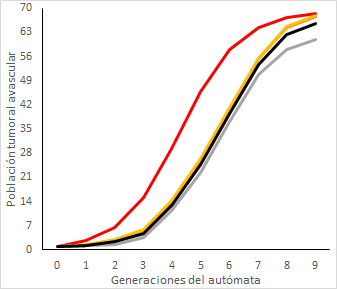
\includegraphics{img/graphs/graph-avascular-simulations-min.png}}
    \scalebox{0.7}{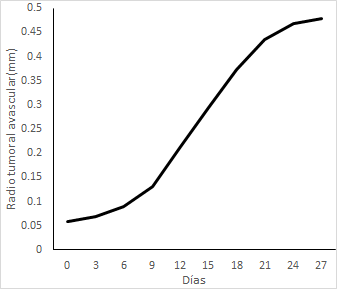
\includegraphics{img/graphs/graph-avascular-simulations-min-r.png}}}\vspace*{-0.2cm}
    \subfigure[Crecimiento promedio $K_a=2$.$222 \times 10^2$]{\scalebox{0.7}{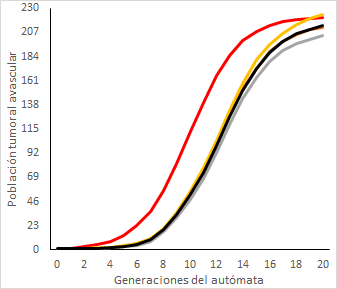
\includegraphics{img/graphs/graph-avascular-simulations-pro.png}}
    \scalebox{0.7}{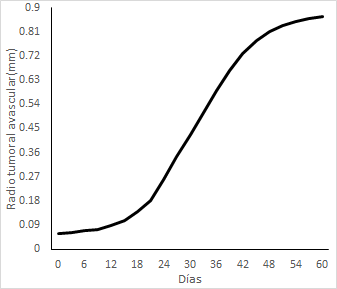
\includegraphics{img/graphs/graph-avascular-simulations-pro-r.png}}}\vspace*{-0.2cm}
    \subfigure[Crecimiento m\'aximo $K_a=4$.$938 \times 10^2$]{\scalebox{0.7}{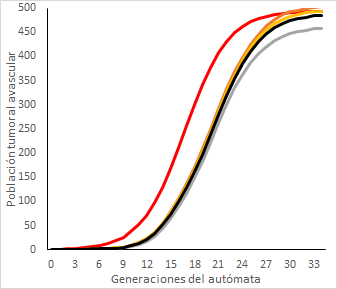
\includegraphics{img/graphs/graph-avascular-simulations-max.png}}
    \scalebox{0.7}{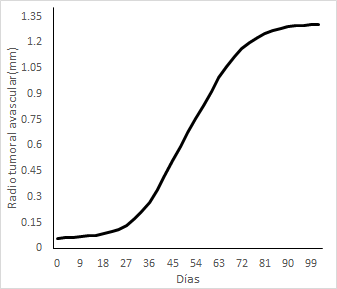
\includegraphics{img/graphs/graph-avascular-simulations-max-r.png}}}\vspace*{-0.2cm}
    \end{center}\vspace*{-0.6cm}
    \caption[Poblaci\'on y radios de un carcinoma ductal infiltrante de crecimiento r\'apido con $\rho_{max}^a=1$ durante la etapa avascular]{Poblaci\'on y radios de un carcinoma ductal infiltrante de crecimiento r\'apido con $\rho_{max}^a=1$ durante la etapa avascular. El resto de par\'ametros se muestran en el cuadro~\ref{table-avascular}. (a,b,c--izquierda) En rojo los valores obtenidos de la soluci\'on de la ley de crecimiento log\'istico, en negro los promedios de la poblaci\'on tumoral y el resto de curvas son varias simulaciones del aut\'omata. (a,b,c--derecha) En negro los promedios del radio tumoral. Tomado de \cite{viabarre2019}.}
    \label{graph-avascular-simulations}
    \end{figure}

%2das

\begin{figure}[p]
    \begin{center}
    \subfigure[Crecimiento m\'inimo $K_a=6$.$944 \times 10^1$]{\scalebox{0.4}{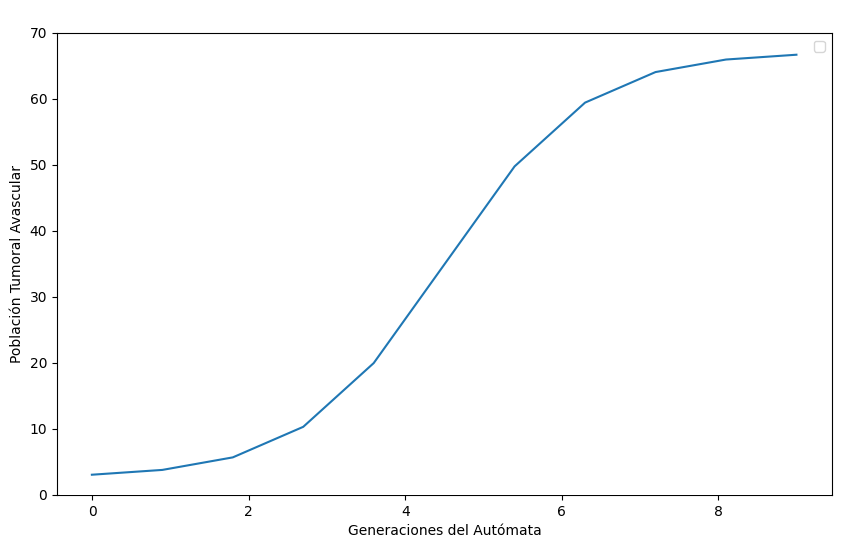
\includegraphics{img/automata/4.4.4.png}}}
    \subfigure[Crecimiento promedio $K_a=2$.$222 \times 10^2$]{\scalebox{0.4}{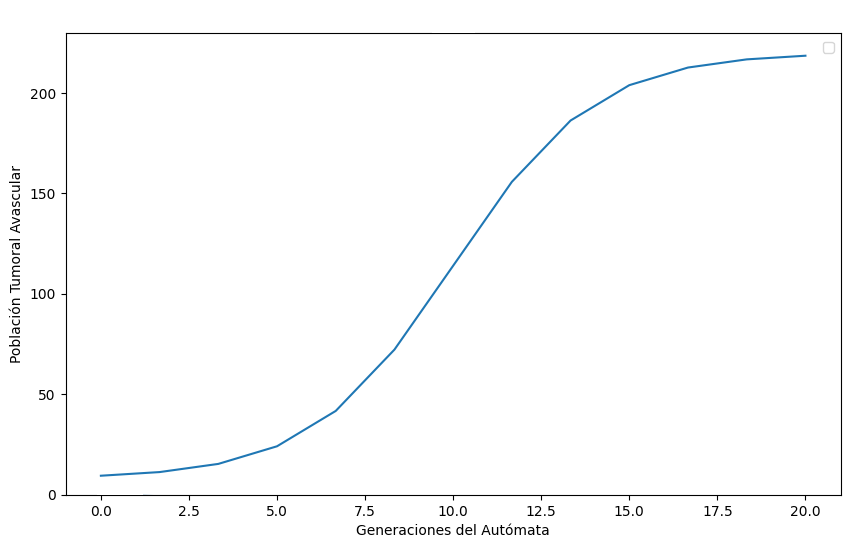
\includegraphics{img/automata/5.5.5.png}}}
    \subfigure[Crecimiento m\'aximo $K_a=4$.$938 \times 10^2$]{\scalebox{0.4}{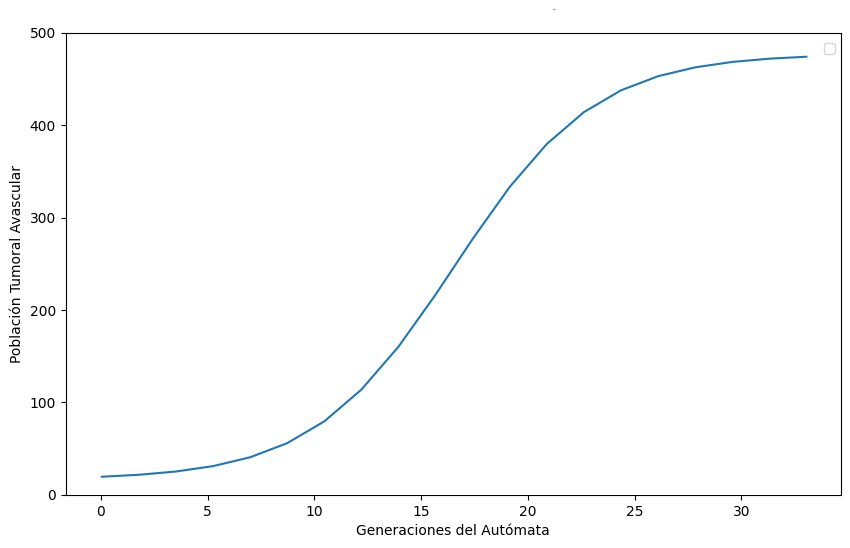
\includegraphics{img/automata/6.6.6.png}}}
    \end{center}\vspace*{-0.6cm}
    \caption[Poblaci\'on y radios de un carcinoma ductal infiltrante de crecimiento lento con $\rho_{max}^a=0$.$1$ durante la etapa avascular]{Poblaci\'on de un carcinoma ductal infiltrante de crecimiento lento con $\rho_{max}^a=1$ durante la etapa avascular.}
    \label{graph-avascular-simulations-1}
    \end{figure}

    \begin{figure}[p]
        \begin{center}
        \subfigure[Crecimiento m\'inimo $K_a=6$.$944 \times 10^1$]{\scalebox{0.7}{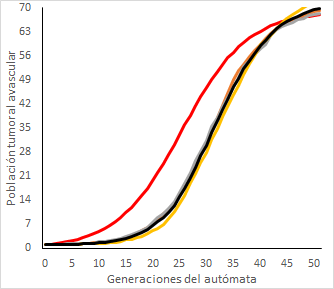
\includegraphics{img/graphs/graph-avascular-simulations-min-1.png}}
        \scalebox{0.7}{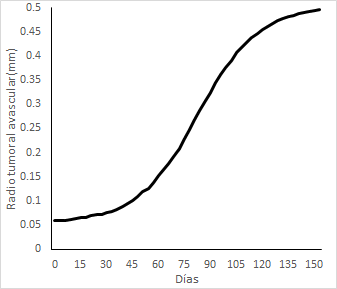
\includegraphics{img/graphs/graph-avascular-simulations-min-r-1.png}}}\vspace*{-0.2cm}
        \subfigure[Crecimiento promedio $K_a=2$.$222 \times 10^2$]{\scalebox{0.7}{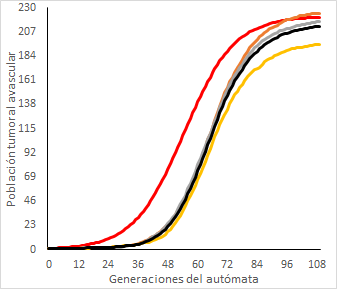
\includegraphics{img/graphs/graph-avascular-simulations-pro-1.png}}
        \scalebox{0.7}{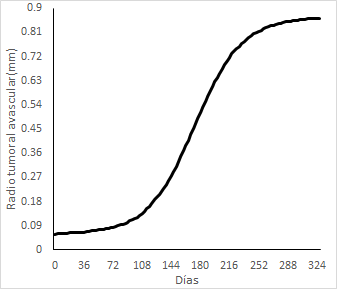
\includegraphics{img/graphs/graph-avascular-simulations-pro-r-1.png}}}\vspace*{-0.2cm}
        \subfigure[Crecimiento m\'aximo $K_a=4$.$938 \times 10^2$]{\scalebox{0.7}{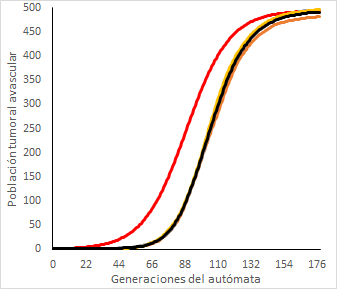
\includegraphics{img/graphs/graph-avascular-simulations-max-1.png}}
        \scalebox{0.7}{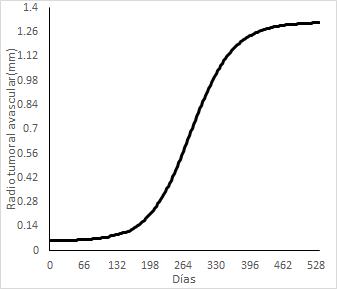
\includegraphics{img/graphs/graph-avascular-simulations-max-r-1.png}}}\vspace*{-0.2cm}
        \end{center}\vspace*{-0.6cm}
        \caption[Poblaci\'on y radios de un carcinoma ductal infiltrante de crecimiento lento con $\rho_{max}^a=0$.$1$ durante la etapa avascular]{Poblaci\'on y radios de un carcinoma ductal infiltrante de crecimiento lento con $\rho_{max}^a=0$.$1$ durante la etapa avascular. El resto de par\'ametros se muestran en el cuadro~\ref{table-avascular-1}. (a,b,c--izquierda) En rojo los valores obtenidos de la soluci\'on de la ley de crecimiento log\'istico, en negro los promedios de la poblaci\'on tumoral y el resto de curvas son varias simulaciones del aut\'omata. (a,b,c--derecha) En negro los promedios del radio tumoral. Tomado de \cite{viabarre2019}.}
        \label{graph-avascular-simulations-1}
        \end{figure}

    Luego, tenemos varias imagenes sobre la simulación del automata celular en etapa avascular:


    En la figura~\ref{fig-avascular-automata} se muestran las visualizaciones de una de las simulaciones del aut\'omata de un carcinoma ductal infiltrante de crecimiento r\'apido durante la etapa avascular. Al tratarse de un carcinoma que constituye un tipo de c\'ancer que surge en el epitelio~(en naranja) se puede apreciar que comienza su desarrollo en esta capa de tejido. Se puede apreciar, adem\'as, la adecuada aplicaci\'on de la regla del crecimiento tumoral definida en la secci\'on~\ref{subsec-celldiv} que establece que durante la etapa avascular un tumor primario no puede penetrar la membrana basal e invadir el estroma~(en gris). En ninguna de las im\'agenes se evidencia esta invasi\'on. La influencia de los vectores de concentraci\'on de nutrientes definen la direcci\'on de la expansi\'on tumoral~(en negro) que se mantiene paralela al epitelio y avanza de forma limitada hacia el lumen~(en blanco). La invasi\'on del estroma tiene lugar durante la etapa vascular del tumor primario y durante las etapas avascular y vascular en tumores secundarios. 
\begin{figure}[!ht]
\begin{center}
\subfigure[Generaci\'on 4]{\scalebox{0.29}{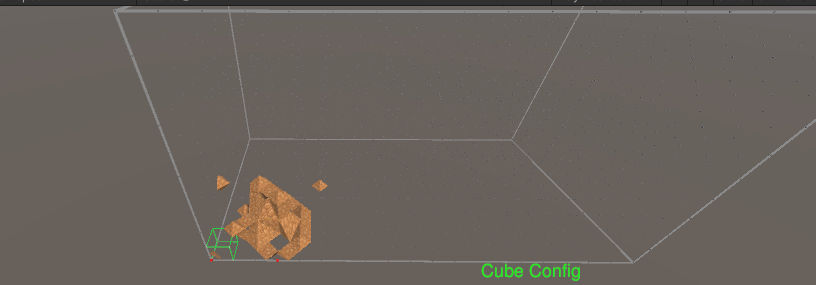
\includegraphics{img/automata/apendix/1.png}}}
\subfigure[Generaci\'on 30]{\scalebox{0.29}{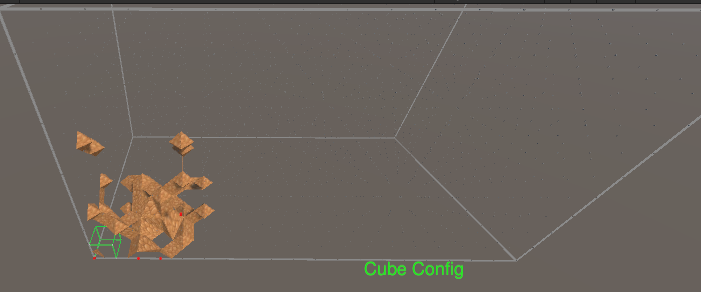
\includegraphics{img/automata/apendix/2.png}}}
\subfigure[Generaci\'on 70]{\scalebox{0.29}{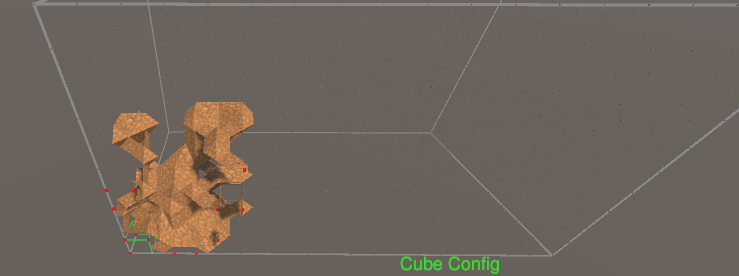
\includegraphics{img/automata/apendix/4.png}}}%\vspace*{-0.25cm}
% \subfigure[Generaci\'on 12]{\scalebox{0.29}{
\includegraphics{img/automata/2019519191641-12.png}}}
% \subfigure[Generaci\'on 16]{\scalebox{0.29}{
\includegraphics{img/automata/2019519191641-16.png}}}
% \subfigure[Generaci\'on 20]{\scalebox{0.29}{
\includegraphics{img/automata/2019519191641-20.png}}}\vspace*{-0.25cm}
\end{center}\vspace*{-0.6cm}
\caption[Visualizaciones de una simulaci\'on del aut\'omata celular de un carcinoma ductal infiltrante de crecimiento r\'apido durante la etapa avascular]{Visualizaciones de una simulaci\'on del aut\'omata celular de un carcinoma ductal infiltrante de crecimiento r\'apido durante la etapa avascular. Las generaciones del aut\'omata mostradas se obtienen mediante los par\'ametros correspondientes con la capacidad de carga promedio~(cuadro~\ref{table-avascular}). El \'area mostrada posee dimensiones $[0,10$.$5]mm \times [0,10$.$5]mm \times [0,10$.$5]mm$ .}
\label{fig-avascular-automata}
\end{figure}


%%%%%%%%%%%%%%%%%%%%%%%%%%%%%%%%%%% Vascular

\section{Crecimiento vascular}
\label{sec-vascular-results}
Este conjunto de par\'ametros de la ley de crecimiento log\'istica describen el desarrollo de un tumor vascular de crecimiento r\'apido. Para ello se utilizan los valores de la poblaci\'on inicial y de las capacidades de carga m\'inimas, promedio y m\'aximas correspondientes con el intervalo de radios vasculares $R_v \in [10, 15]mm$ y una probabilidad m\'axima vascular $\rho_{max}^v=1$ como se muestra en el cuadro~\ref{table-vascular}. La poblaci\'on inicial utilizada es la capacidad de carga avascular promedio, es decir, $P_0^v = K_a = 2$.$222 \times 10^2$. Los resultados provenientes de las simulaciones con los par\'ametros del cuadro~\ref{table-vascular} se muestran en las gr\'aficas~\ref{graph-vascular-simulations}. El an\'alisis de los resultados presentados se lleva a cabo en la secci\'on~\ref{sec-growth-validation}.
\begin{table}[!ht]
\begin{center}
\scalebox{0.9}{\begin{tabular}{|p{2.1cm}|p{14.5cm}|}\hline
\emph{M\'inimo} & $P_0^v=2$.$222 \times 10^2$, $K_v=2$.$778 \times 10^4$, $r_v=1$.$44 \times 10^{-4}$, $\Delta t=5$.$401 \times 10^2$, generaciones del aut\'omata: $121$~($363$ d\'ias).\\\hline
\emph{Promedio} & $P_0^v=2$.$222 \times 10^2$, $K_v=5$.$556 \times 10^4$, $r_v=7$.$199 \times 10^{-5}$, $\Delta t=7$.$665 \times 10^2$, generaciones del aut\'omata: $201$~($603$ d\'ias).\\\hline
\emph{M\'aximo} & $P_0^v=2$.$222 \times 10^2$, $K_v=1$.$111 \times 10^5$, $r_v=3$.$6 \times 10^{-5}$, $\Delta t=1$.$079 \times 10^3$, generaciones del aut\'omata: $321$~($963$ d\'ias).\\\hline
\end{tabular}}\vspace*{-0.6cm}
\end{center}
\caption[Par\'ametros del desarrollo de un carcinoma ductal infiltrante de crecimiento r\'apido durante la etapa vascular]{Par\'ametros del desarrollo de un carcinoma ductal infiltrante de crecimiento r\'apido durante la etapa vascular.}
\label{table-vascular}
\end{table}

%3ra
\begin{figure}[p]
    \begin{center}
    \subfigure[Crecimiento m\'inimo $K_a=6$.$944 \times 10^1$]{\scalebox{0.4}{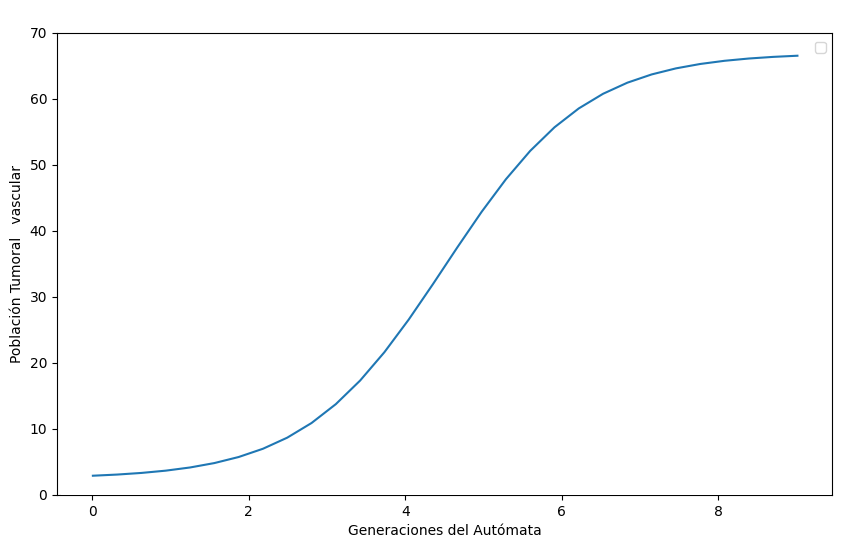
\includegraphics{img/automata/7.7.7.png}}}
    \subfigure[Crecimiento promedio $K_a=2$.$222 \times 10^2$]{\scalebox{0.4}{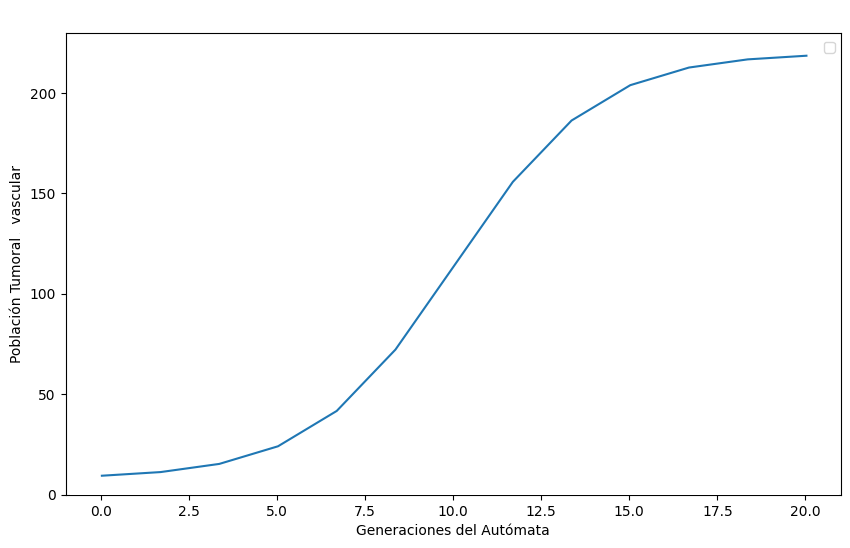
\includegraphics{img/automata/8.8.8.png}}}
    \subfigure[Crecimiento m\'aximo $K_a=4$.$938 \times 10^2$]{\scalebox{0.4}{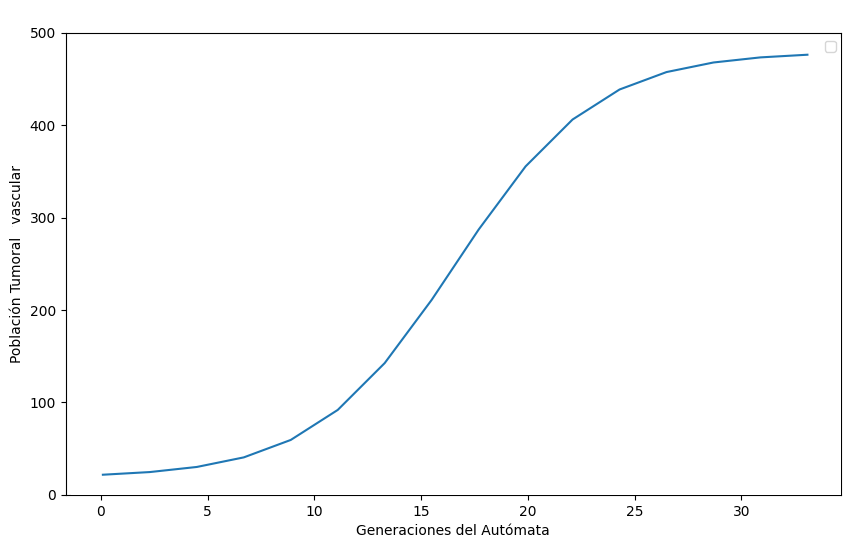
\includegraphics{img/automata/9.9.9.png}}}
    \end{center}\vspace*{-0.6cm}
    \caption[Poblaci\'on  de un carcinoma ductal infiltrante de crecimiento lento con $\rho_{max}^a=0$.$1$ durante la etapa avascular]{Poblaci\'on de un carcinoma ductal infiltrante de crecimiento r\'apido con $\rho_{max}^v=1$ durante la etapa vascular.}
    \label{graph-avascular-simulations-1}
    \end{figure}

\begin{figure}[p]
\begin{center}
\subfigure[Crecimiento m\'inimo $K_v=2$.$778 \times 10^4$]{\scalebox{0.7}{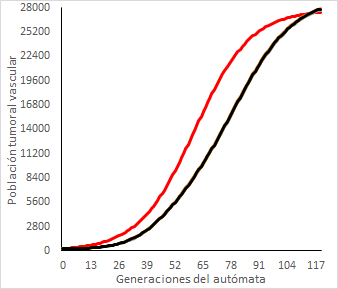
\includegraphics{img/graphs/graph-vascular-simulations-min.png}}
\scalebox{0.7}{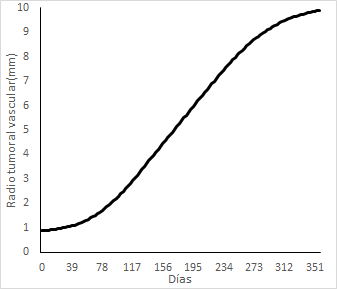
\includegraphics{img/graphs/graph-vascular-simulations-min-r.png}}}\vspace*{-0.2cm}
\subfigure[Crecimiento promedio $K_v=5$.$556 \times 10^4$]{\scalebox{0.7}{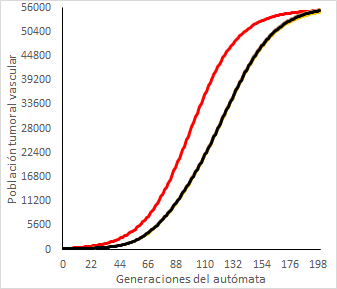
\includegraphics{img/graphs/graph-vascular-simulations-pro.png}}
\scalebox{0.7}{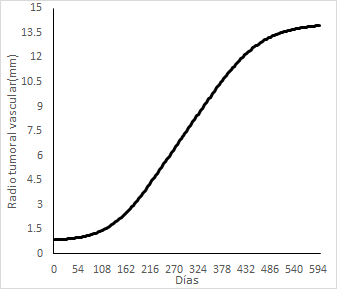
\includegraphics{img/graphs/graph-vascular-simulations-pro-r.png}}}\vspace*{-0.2cm}
\subfigure[Crecimiento m\'aximo $K_v=1$.$111 \times 10^5$]{\scalebox{0.7}{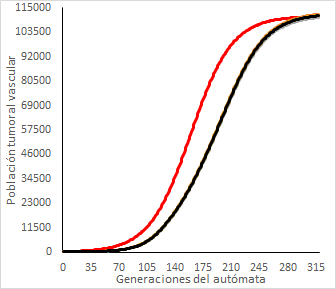
\includegraphics{img/graphs/graph-vascular-simulations-max.png}}
\scalebox{0.7}{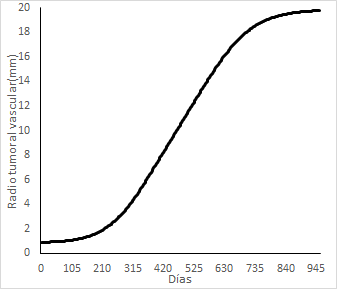
\includegraphics{img/graphs/graph-vascular-simulations-max-r.png}}}\vspace*{-0.2cm}
\end{center}\vspace*{-0.6cm}
\caption[Poblaci\'on y radios de un carcinoma ductal infiltrante de crecimiento r\'apido con $\rho_{max}^v=1$ durante la etapa vascular]{Poblaci\'on y radios de un carcinoma ductal infiltrante de crecimiento r\'apido con $\rho_{max}^v=1$ durante la etapa vascular. El resto de par\'ametros se muestran en el cuadro~\ref{table-vascular}. (a,b,c--izquierda) En rojo los valores obtenidos de la soluci\'on de la ley de crecimiento log\'istico, en negro los promedios de la poblaci\'on tumoral y el resto de curvas son varias simulaciones del aut\'omata. (a,b,c--derecha) En negro los promedios del radio tumoral. Tomado de \cite{viabarre2019}.}
\label{graph-vascular-simulations}
\end{figure}

\section{Validaci\'on del crecimiento tumoral}
\label{sec-growth-validation}

Se puede observar, de los resultados de ~\ref{graph-avascular-simulations-mine} que se obtiene una curva parecida a la descrita en \cite{book} presente en otros modelos de la literatura que utilizan otras ecuaciones de crecimiento como Gompertz~\cite{kansal,dormann,kansal2,kansal3}. Cabe destacar que el modelo devuelve valores biol\'ogicamente realistas. A pesar de no contar con muchas c\'elulas presenta una curva de crecimiento que acierta tanto en el tiempo como en la cantidad de c\'elulas cancer\'igenas en cierto instante de tiempo presentes en la simulaci\'on. Los casos mostrados anteriormente demuestran que el modelo es capaz de reconstruir el desarrollo tumoral para ambas etapas en un per\'iodo de tiempo arbitrario.

Para analizar el radio y las poblacioes se hace necesario tener en cuenta el escalado de la simulación, se hace muy d\'ificil realizar comparaciones con resultados de la literatura. Teniendo una escala m\'as realista de 1:1 se podr\'ian contabilizar mejor la cantidad de c\'elulas, ya que actualmente se est\'a asumiendo que existen muchas c\'elulas que comparten un mismo estado en cada rejilla de la grilla. Luego de realizar varios an\'alisis se obtuvo que al menos el 46\% de las veces el radio suele coincidir aproximadamente con los resultados presentes en la literatura, obteni\'endose valores del radio de 0.5mm para la etapa avascular y partiendo de este valor
obtener un radio de 10mm para la etapa vascular.

% Insertar Imagen

\section*{C\'elulas migratorias y met\'astasis}

Se presentan resultados sobre la migración y met\'astasis a un tumor secundario. En las im\'agenes se puede presenciar como las c\'elulas tumorales de desprenden del tumor principal y van invadiendo al \'organo secundario formando una micrometástasis.

% Insertar imagenes
\begin{figure}[p]
    \begin{center}
    \subfigure[Generaci\'on 125]{\scalebox{0.23}{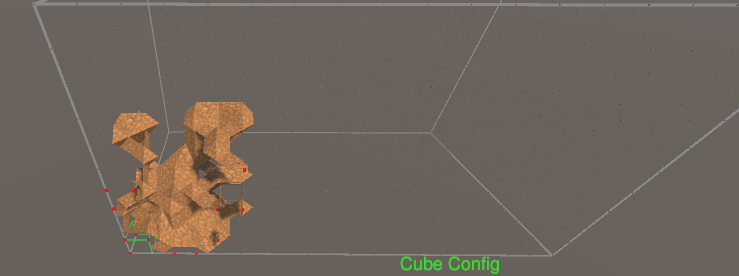
\includegraphics{img/automata/apendix/4.png}}}
    \subfigure[Generaci\'on 150]{\scalebox{0.23}{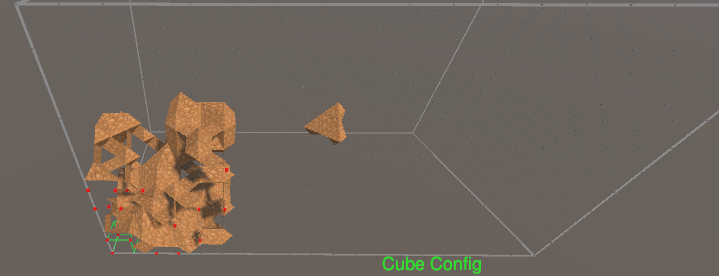
\includegraphics{img/automata/apendix/5.png}}}
    
    \subfigure[Generaci\'on 175]{\scalebox{0.23}{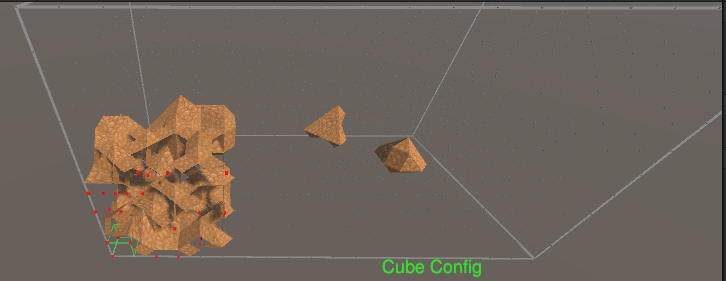
\includegraphics{img/automata/apendix/6.png}}}
    \subfigure[Generaci\'on 200]{\scalebox{0.23}{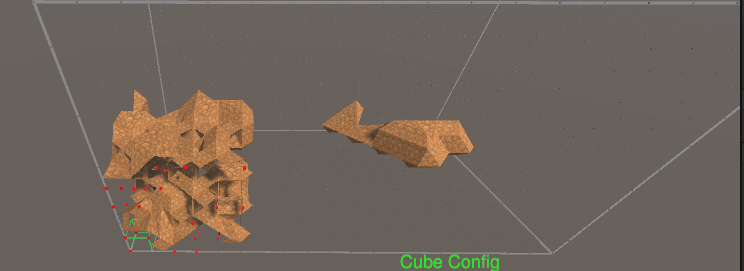
\includegraphics{img/automata/apendix/7.png}}}
    % \scalebox{0.23}{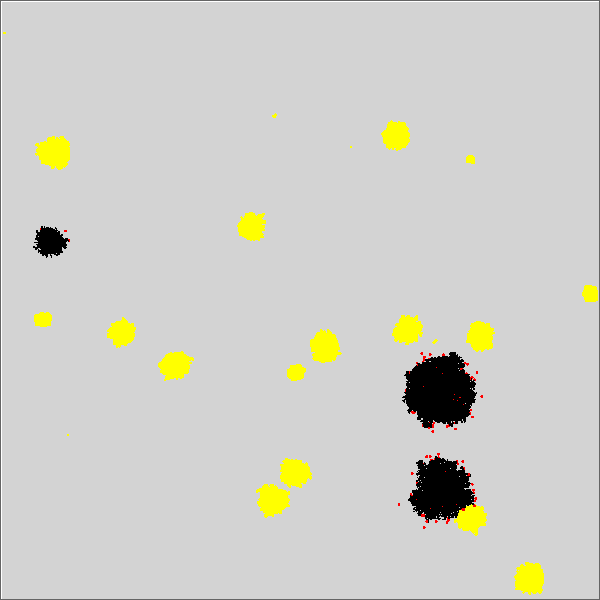
\includegraphics{img/automata/meta/201952320435-200-Secondary.png}}}\vspace*{-0.2cm}
    
    % \subfigure[Generaci\'on 225]{\scalebox{0.23}{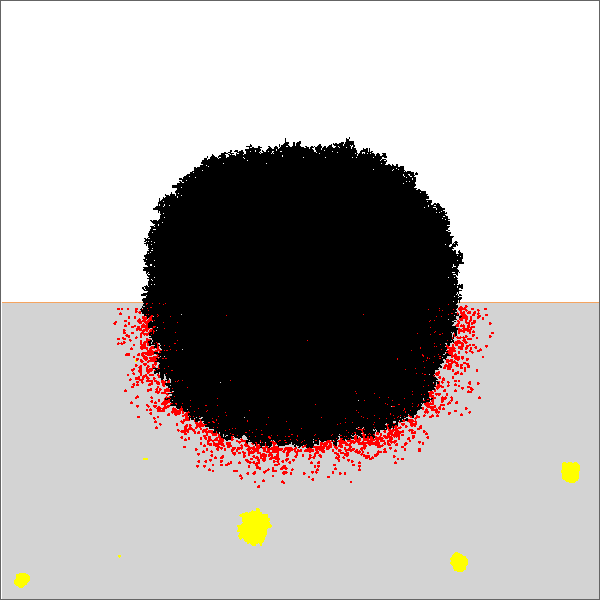
\includegraphics{img/automata/meta/201952320435-225-Primary.png}}
    % \scalebox{0.23}{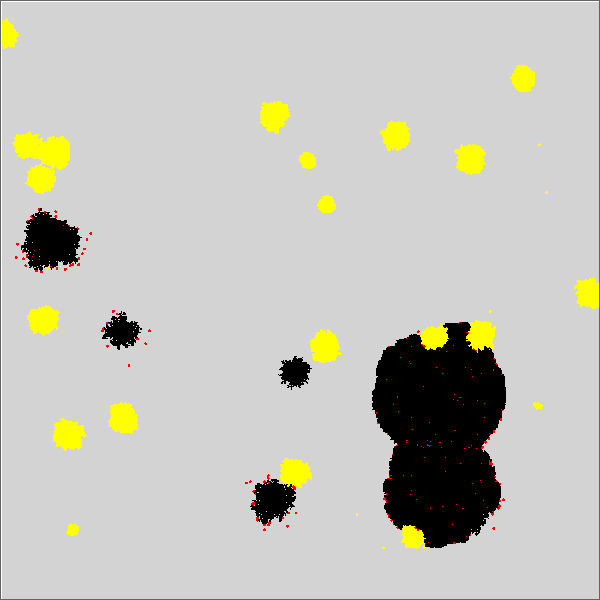
\includegraphics{img/automata/meta/201952320435-225-Secondary.png}}}
    % \subfigure[Generaci\'on 250]{\scalebox{0.23}{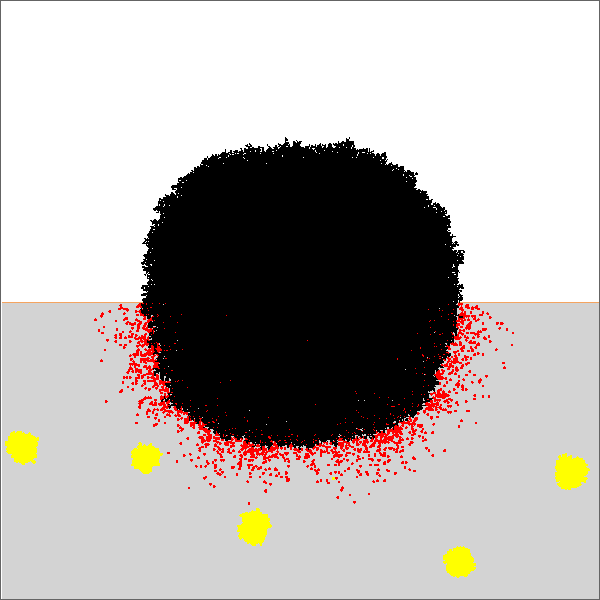
\includegraphics{img/automata/meta/201952320435-250-Primary.png}}
    % \scalebox{0.23}{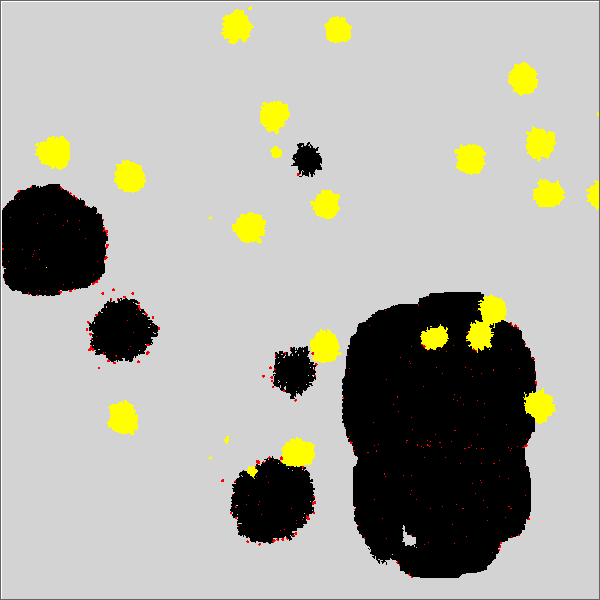
\includegraphics{img/automata/meta/201952320435-250-Secondary.png}}}\vspace*{-0.2cm}
    
    % \subfigure[Generaci\'on 275]{\scalebox{0.23}{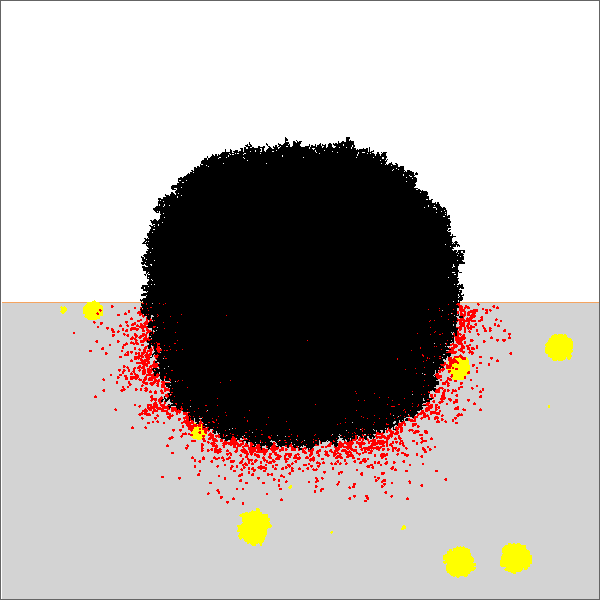
\includegraphics{img/automata/meta/201952320435-275-Primary.png}}
    % \scalebox{0.23}{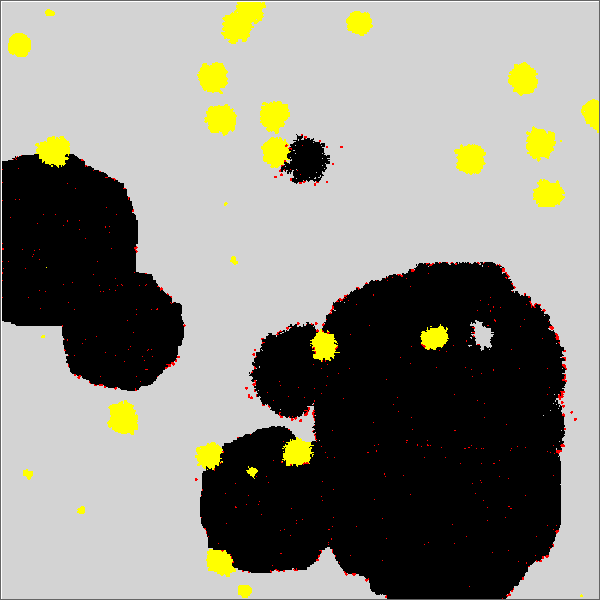
\includegraphics{img/automata/meta/201952320435-275-Secondary.png}}}
    % \subfigure[Generaci\'on 300]{\scalebox{0.23}{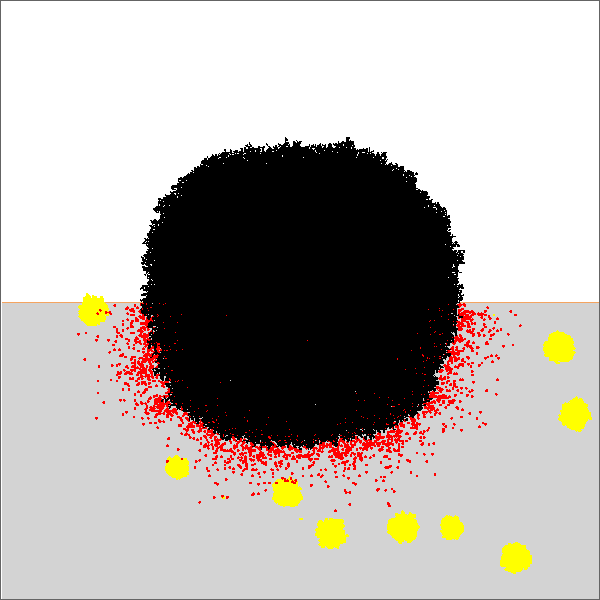
\includegraphics{img/automata/meta/201952320435-300-Primary.png}}
    % \scalebox{0.23}{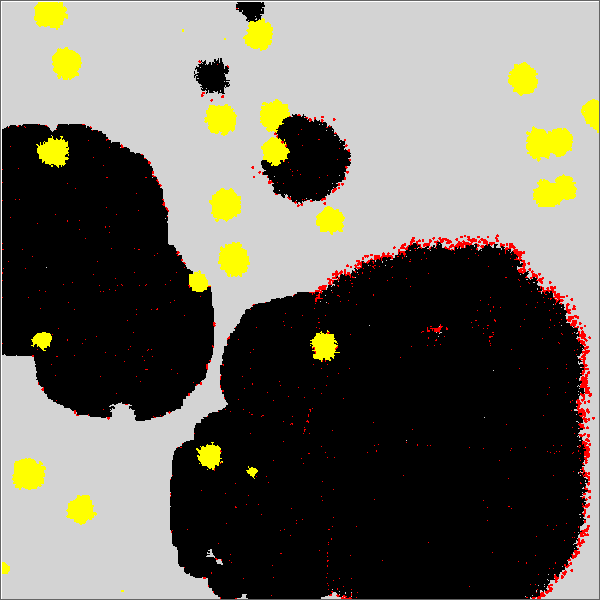
\includegraphics{img/automata/meta/201952320435-300-Secondary.png}}}\vspace*{-0.2cm}
    \end{center}\vspace*{-0.6cm}
    \caption[Visualizaciones de una simulaci\'on del aut\'omata celular del ciclo vital del c\'ancer donde el tumor primario posee un alto potencial metast\'asico]{Visualizaciones de una simulaci\'on del aut\'omata celular del ciclo vital del c\'ancer donde el tumor primario posee un alto potencial metast\'asico y la localizaci\'on destino se corresponde con los pulmones. El tumor de mayor \'area es el principal y el de menor \'area es el secundario que est\'a llevando a cabo la met\'astasis. El \'area mostrada para cada localizaci\'on posee dimensiones $[0,52$.$5]mm \times [0,52$.$5]mm \times [0,52$.$5]mm$.}
    \label{fig-full-automata}
    \end{figure}